\chapter{Grundlagen}\label{sec:basics}

In diesem Kapitel werden Themen vorgestellt, die für das generelle Verständnis der Arbeit benötigt werden. Dafür wird zunächst die grobe Funktionsweise des menschlichen Auges beschrieben. Weiter wird vorgestellt, welche verschiedenen Methoden es gibt, um die Blickrichtung eines Menschen zu bestimmen. Anschließend werden Convolutional Neural Networks vorgestellt. Am Ende werden Metriken präsentiert, die für die Evaluation dieser Arbeit verwendet werden.

\section{Funktionsweise des menschlichen Auges}\label{sec:basics:eye}

Um unsere Umwelt optisch wahrnehmen zu können, wandelt das menschliche Auge Licht in elektrische Signale um. Das Licht fällt dabei zunächst durch die Pupille des Auges, wird im Auge gebrochen und auf die Netzhaut \cite[S.~12]{book:eyes} projiziert. Auf der Netzhaut befinden sich lichtempfindliche Zellen, die das einfallende Licht in elektrische Signale umwandeln können. Man unterscheidet zwischen Zapfen und Stäbchen. Die Zapfen sind die Zellen, mit denen der Mensch Farben wahrnehmen kann. Die Stäbchen hingegen können auch schwache Lichtreize wahrnehmen und ermöglichen so das Sehen bei schlechten Lichtverhältnissen. Über den Sehnerv werden die Signale an den visuellen Cortex weitergeleitet. So nennt man den Teil des menschlichen Gehirns, der die elektrischen Signale zu einem Bild zusammensetzt \cite[S.~13]{book:eyes}\cite{paper:cnn}. 

Auf der Netzhaut gibt es einen Bereich, in dem besonders viele Zapfen vorhanden sind. Diesen Bereich nennt man den gelben Fleck \cite[S.~13]{book:eyes}. Um etwas scharf sehen zu können, muss das Auge so bewegt werden, dass das Licht direkt auf diesen Bereich fällt. Die Linie zwischen dem Punkt, den das Auge dabei fixiert, und dem gelben Fleck wird Sichtlinie oder visuelle Achse genannt und gibt die Blickrichtung eines Menschen an \cite{paper:basic:eye:tracking}. Daneben gibt es noch die Blicklinie oder optische Achse, die die Verbindung der Pupille mit dem Zentrum des Augapfels beschreibt \cite{paper:basic:eye:tracking}.

Bei der dreidimensionalen Betrachtung der Blickrichtung einer Person spielt neben den Augenbewegungen auch die Kopfdrehung eine Rolle. Diese können als Drehung um drei verschiedene Achsen beschrieben werden. Die erste Achse ist die Querachse, auch horizontale Achse genannt. Der Winkel, um den der Kopf oder das Auge um diese Achse gedreht wird, wird als \textit{Pitch} bezeichnet. Dieser beschreibt die Rotation nach oben und unten. Dann gibt es die Vertikalachse. Sie beschreibt die Drehung nach links und rechts. Die Drehung um diese Achse wird mit dem \textit{Yaw}-Winkel angegeben. Die dritte Achse ist die Längsachse, die das Kippen des Kopfes nach links und rechts beschreibt. Der Winkel, um den der Kopf dabei gekippt wird, wird als \textit{Roll}-Winkel bezeichnet. Die Achsen sind in der Abbildung \ref{fig:basics:axis} dargestellt.

\begin{figure}[]
    \centering
    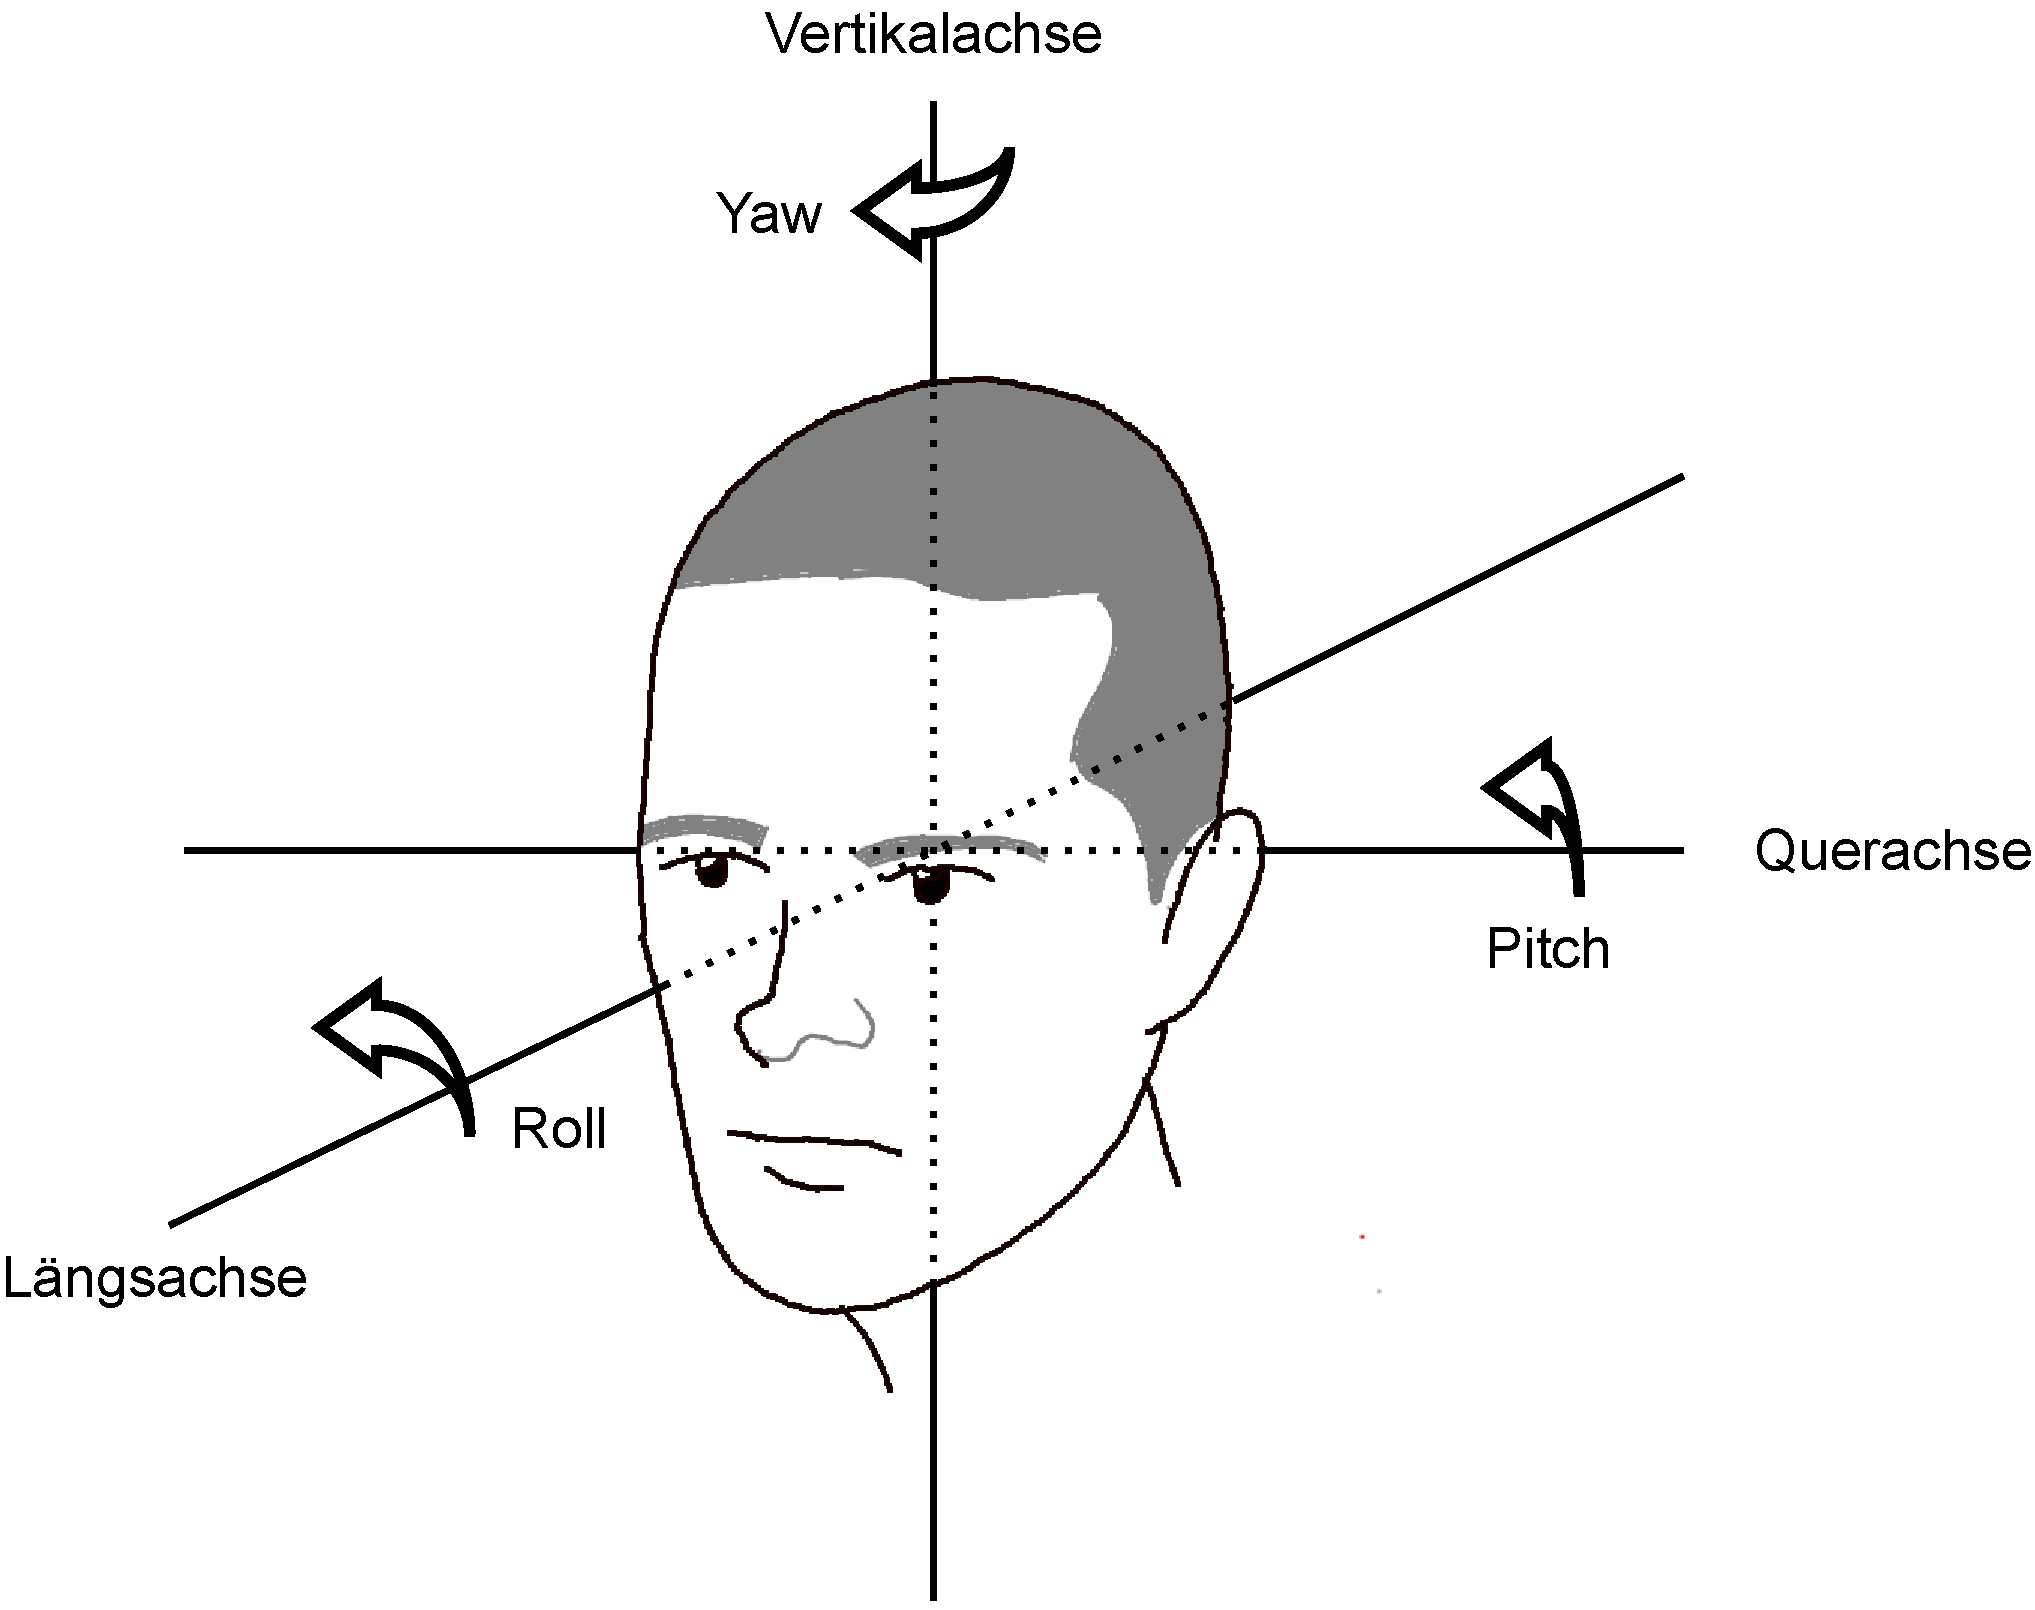
\includegraphics[width=0.8\linewidth]{basics/head.pdf}
    \caption{Darstellung der Quer-, Längs- und Vertikalachse des Kopfes eines Menschen. Quelle: Abbildung nach \cite{paper:eye-coordinates}}
    \label{fig:basics:axis}
\end{figure}

\section{Methoden zur Bestimmung der Blickrichtung}

In diesem Abschnitt werden verschiedene Methoden vorgestellt, die es ermöglichen die Blickrichtung einer Person zu bestimmen.

Das erste Verfahren ist die \textit{Elektrookulographie}. Bei diesem Verfahren werden die Augenbewegungen gemessen, um die Blickrichtung eines Menschen zu bestimmen. Zur Messung der Augenbewegung werden Elektroden links und rechts bzw. oberhalb und unterhalb der Augen angebracht. Aus der zwischen diesen Elektroden abgeleiteten Spannung können Rückschlüsse auf die Augenbewegung gezogen werden. Diese Methode ist daher nur für spezielle Anwendungsfälle geeignet \cite{paper:basics:survey}\cite[S.~70]{book:eyes}. 

Weiter lässt sich die Blickrichtung mittels \textit{3D Eye Model Recovery-Based} Methoden \cite{paper:basics:survey} bestimmen. Bei diesem Verfahren wird mithilfe von zusätzlicher Hardware wie Infrarotkameras ein dreidimensionales geometrisches Modell des Auges rekonstruiert. Für die Konstruktion dieses Modells werden jedoch personenspezifische Werte des Auges benötigt, die durch eine Kalibrierung ermittelt werden müssen. Ein solches Verfahren liefert genaue Vorhersagen über die Blickrichtung, kann aber immer nur für eine Person verwendet werden. Für jede weitere Person muss die Kalibrierung erneut durchgeführt werden. Außerdem wird, wie bereits erwähnt, zusätzliche Hardware benötigt, was die Einsatzmöglichkeiten dieses Verfahrens ebenfalls limitiert \cite{paper:basics:survey}. 

Bei \textit{2D Feature Regression-Based Methoden} \cite{paper:basics:survey} werden ebenfalls mit zusätzlicher Hardware geometrische Eigenschaften des Auges erfasst. Diese Eigenschaften können z.B. das Zentrum der Pupille oder die Reflektion von Lichtquellen auf der Hornhaut des Auges sein. Anhand der erkannten Merkmale, kann dann mit einer Regressionsfunktion bestimmt werden, wohin eine Person sieht \cite{paper:basics:survey}.

Es gibt Verfahren, die ohne zusätzliche Hardware und nur mit einer Kamera auskommen. Dabei handelt es sich um die \textit{Deep Learning Appearance-Based} \cite{paper:basics:survey} Verfahren. Sie nutzen das Bild einer Person, um Informationen über die Blickrichtung der Person zu extrahieren und darauf aufbauend die Blickrichtung vorherzusagen. Diese Verfahren benötigen jedoch eine große Menge an Trainingsdaten, um eine zuverlässige Blickrichtungsbestimmung zu ermöglichen. Dabei ist die Wahl des Datensatzes für den jeweiligen Anwendungsfall entscheidend. In der Regel sind die Ergebnisse eines solchen Ansatzes nicht so genau wie Verfahren, die auf zusätzlicher Hardware basieren \cite{paper:basics:survey}. Sie benötigen jedoch keine Kalibrierung, sind kostengünstiger und können ohne Einschränkungen eingesetzt werden. Ein weiterer Vorteil ist, dass sich die Personen bei solchen Verfahren uneingeschränkt bewegen können.

\section{Convolutional Neural Networks}

Eine Architektur von Neuronalen Netzen, die für Deep Learning Methoden verwendet werden kann, sind \textit{Convolutional Neural Networks}. \cite{diplom:matthes, paper:cnn}. Diese eignen sich sehr gut zur Erkennung von Mustern in Bildern \cite{diplom:matthes, paper:eth-xgaze, paper:mpiigaze, paper:rt_gene, paper:gaze360}. Als Eingabe dient ein Raster von Pixelwerten der zu verarbeitenden Bilder. Der generelle Aufbau von Convolutional Neural Networks besteht im Wesentlichen aus mehreren \textit{Convolution}-Schichten, denen jeweils eine \textit{Pooling}-Schicht \cite{paper:cnn} folgt. In den Convolution-Schichten werden Filter verwendet, um Muster in den Bilddaten zu erkennen. Ein solcher Filter ist eine kleine Matrix, die über das Raster der Pixelwerte verschoben wird und eine Punktprodukt-Operation mit den Pixelwerten durchführt. So können in diesen Schichten Muster wie Kanten und andere visuelle Informationen extrahiert werden \cite{diplom:matthes, paper:cnn}. In der anschließenden Pooling-Schicht wird die Dimensionalität der Daten reduziert, wobei die wichtigen Informationen erhalten bleiben \cite{paper:cnn}. In einer abschließenden \textit{Fully Connected}-Schicht werden die extrahierten Merkmale der vorhergehenden Schichten verwendet, um eine Klassifikation vorzunehmen, wie z.B. die ermittelte Blickrichtung der abgebildeten Person.

\section{Metriken für binäre Entscheidungen}

In diesem Abschnitt werden Metriken vorgestellt, die für die Evaluation dieser Arbeit verwendet werden. Die grundlegende Entscheidung, die in dieser Arbeit getroffen werden muss, ist, zu welchen Zeitpunkten die Radfahrenden auf ihr Smartphone schauen. Dabei handelt es sich um eine binäre Entscheidung, d.h. die Person schaut auf das Smartphone oder die Person schaut nicht auf das Smartphone. Zur Bewertung dieser Entscheidung wird eine Ground Truth benötigt, die den tatsächlichen Zustand zu einem bestimmten Zeitpunkt repräsentiert. Die Ground Truth kann in positive und negative Instanzen unterteilt werden. Die positiven Instanzen sind in diesem Beispiel die Zeitpunkte, zu denen die Person auf das Smartphone schaut. Die negativen Instanzen sind die Zeitpunkte, zu denen die Person nicht auf das Smartphone schaut. Anhand der Ground Truth kann jede Vorhersage, einer von vier Klassen zugeordnet werden \cite{diplom:matthes}.

Zunächst gibt es die \textit{True Positives} ($TP$). Eine Entscheidung gehört zu dieser Klasse, wenn richtig vorhergesagt wurde, dass der positive Fall eingetreten ist. In diesem Fall würde das bedeuten, dass richtig erkannt wurde, dass die Person auf das Smartphone schaut. Analog dazu gibt es die \textit{True Negatives} ($TN$). Diese geben in diesem Beispiel an, dass richtig vorhergesagt wurde, dass die Person nicht auf das Smartphone schaut. Für falsche Entscheidungen gibt es die \textit{False Positives} ($FP$) und die \textit{False Negatives} ($FN$). Zu den \textit{False Positives} gehören die Entscheidungen, bei denen erkannt wurde, dass die Person auf das Smartphone schaut, die Person aber zu diesem Zeitpunkt nicht auf das Smartphone geschaut hat. Die \textit{False Negatives} hingegen beschreiben, dass nicht erkannt werden konnte, dass die Person zu einem bestimmten Zeitpunkt auf das Smartphone geschaut hat.

Aus dieser vier Klassen lassen sich die Metriken \textit{Recall} und \textit{Precision} bestimmen. Der \textit{Recall} ist das Verhältnis der richtig vorhergesagten positiven Instanzen ($TP$) zur Gesamtzahl der positiven Instanzen in der Ground Truth. Die Gesamtzahl kann als Summe der \textit{True Positives} und der \textit{False Negatives} definiert werden \cite{diplom:matthes}. Der Recall kann somit wie folgt berechnet werden:

\[
\text{Recall} = \frac{TP}{TP + FN}
\]

Die Metrik \textit{Precision} beschreibt, wie viele positive Vorhersagen richtig waren \cite{diplom:matthes}. Dabei wird das Verhältnis der \textit{True Positives} zur Summe der \textit{True Positives} und \textit{False Positives} berechnet:

\[
\text{Precision} = \frac{TP}{TP + FP} \\
\]

Aus diesen beiden Metriken lässt sich die Metrik \textit{F1-Score} bestimmen. Diese Metrik ermöglicht es, \textit{Precision} und \textit{Recall} in einer gemeinsamen Metrik \cite{diplom:matthes} abzubilden. Der \textit{F1-Score} beschreibt dabei das harmonische Mittel zwischen den beiden Metriken.

\[
\text{F1-Score} = 2 \cdot \left( \frac{\text{Precision} \cdot \text{Recall}}{\text{Precision} + \text{Recall}} \right)
\]

Der kleinstmögliche Wert des \textit{F1-Scores} ist 0. Tritt dieser Fall ein, bedeutet das, dass entweder \textit{Precision} oder \textit{Recall} gleich 0 sind. Der bestmögliche Wert für den \textit{F1-Score} ist 1, was bedeutet, dass bei der Bestimmung keine falsche Vorhersage getroffen wurde.

\section{Zusammenfassung}

In diesem Kapitel wurden die wichtigsten Grundlagen für das Verständnis der Arbeit erläutert. Zunächst wurde die Funktionsweise des Auges dargestellt. Darauf aufbauend konnte erklärt werden, dass die Blickrichtung eines Menschen durch die Linie zwischen Pupille, gelbem Fleck und dem betrachteten Objekt definiert werden kann. Weiterhin wurde gezeigt, wie die Bewegung der Augen bzw. des Kopfes eines Menschen durch Drehung um drei verschiedene Achsen mit den Winkeln \textit{Pitch}, \textit{Yaw} und \textit{Roll} angegeben werden kann.  

Anschließend wurden verschiedene Methoden zur Bestimmung der Blickrichtung vorgestellt.  Diese lassen sich im Wesentlichen in zwei Kategorien einteilen: Methoden, die auf zusätzlicher Hardware basieren und Methoden, die mittels Deep Learning auf Basis eines Kamerabildes arbeiten. Für diese Deep Learning Appearance-Based Methoden eignen sich insbesondere Convolutional Neural Networks, deren Funktionsweise ebenfalls vorgestellt wurde. 

Abschließend wurden die Metriken \textit{Recall}, \textit{Precision} und \textit{F1-Score} vorgestellt, die zur Evaluation dieser Arbeit verwendet werden. 



